%% SoftwareX Original Software Publication -- fwhFoam
%% Based on Elsevier's official softwarex-osp-template.tex (elsarticle).

\documentclass[preprint,12pt,a4paper]{elsarticle}

\usepackage{amssymb}
\usepackage{amsmath}
\usepackage{booktabs}
\usepackage{hyperref}
\setlength{\parindent}{0pt}

\journal{SoftwareX}

\begin{document}

\begin{frontmatter}

\title{fwhFoam: A Ffowcs Williams--Hawkings solver with on-surface
acoustic source localization for OpenFOAM}

\author[dlr]{Sparsh Sharma}
\ead{sparsh.sharma@dlr.de}
\address[dlr]{German Aerospace Center (DLR), Germany}

\begin{abstract}
\texttt{fwhFoam} is an open-source aeroacoustic post-processing library for
OpenFOAM. It predicts far-field sound with Farassat's formulation~1A of the
Ffowcs Williams--Hawkings equation for permeable and impermeable integration
surfaces through one code path, with a uniform mean flow handled in closed
form. From the same surface data it also computes the surface sound-power
density $\sigma$ of the diffraction-filter theory of Delfs \& Ruck, which
maps where the radiated sound originates on the surface, subject to the
power identity $\oint\sigma\,dS = P_\mathrm{far\text{-}field}$. Far-field
predictions match analytic monopole, dipole and convected-monopole solutions
to $\sim$0.1\,\%, and the $\sigma$ identity is verified to a few tenths of a
percent on analytic sources.
\end{abstract}

\begin{keyword}
Aeroacoustics \sep Ffowcs Williams--Hawkings \sep Acoustic source
localization \sep Surface sound-power density \sep OpenFOAM
\end{keyword}

\end{frontmatter}

%% ------------------------------------------------------------------
\section*{Required Metadata}

\section*{Current code version}

\begin{table}[!h]
\begin{tabular}{|l|p{5.4cm}|p{6.2cm}|}
\hline
\textbf{Nr.} & \textbf{Code metadata description} & \textbf{Value} \\
\hline
C1 & Current code version & v1.0.0 \\
\hline
C2 & Permanent GitHub link to code/repository & \url{https://github.com/Sparsh-Sharma/fwhFoam} \\
\hline
C3 & Legal Code License & GPL-3.0-or-later \\
\hline
C4 & Code versioning system used & git \\
\hline
C5 & Software code languages, tools, and services used & C++ (C++14), Python~3, OpenFOAM (\texttt{wmake}) \\
\hline
C6 & Compilation requirements, operating environments \& dependencies & OpenFOAM~v2306; C++14 compiler; Python~$\ge$3.9 with NumPy and SciPy \\
\hline
C7 & Link to developer documentation/manual & \texttt{README.md}, \texttt{doc/theory.md}, \texttt{doc/fwh-data-format.md} in the repository \\
\hline
C8 & Support email for questions & sparsh.sharma@dlr.de \\
\hline
\end{tabular}
\caption{Code metadata (mandatory)}
\end{table}

%% ------------------------------------------------------------------
\section{Motivation and significance}
\label{sec:motivation}

Aerodynamically generated sound is a central concern in the design of
aircraft, rotors, wind turbines, ground vehicles and cooling fans. Direct
computation of the acoustic field together with the flow is prohibitively
expensive for most engineering configurations, because the acoustic
fluctuations are orders of magnitude smaller than the hydrodynamic ones and
the far field lies many wavelengths from the source. The established remedy
is an \emph{acoustic analogy}: the near-field unsteady flow is computed by
scale-resolving CFD, and an integral formulation propagates the sound to
far-field observers at negligible additional cost. The Ffowcs
Williams--Hawkings (FW-H) equation~\cite{fwh1969} is the most general such
analogy, and in its permeable (porous-surface) form~\cite{difrancescantonio1997,
brentner1998} accounts for volume (quadrupole) sources by enclosing them
within an off-body integration surface. Farassat's formulation~1A~\cite{farassat2007}
is its standard time-domain realization.

Mature open-source FW-H implementations for OpenFOAM already exist; the most
established is \texttt{libAcoustics}~\cite{epikhin2015}, providing Curle,
Farassat~1A (permeable and impermeable) and a wind-tunnel formulation.
\texttt{fwhFoam} does not aim to replace such tools on far-field prediction,
and we claim no novelty for the FW-H formulation, which is standard. It makes
a compact, verifiable FW-H capability openly available with a reproducible
verification and convergence suite. In addition, it couples the far-field
prediction with on-surface source localization: the same permeable-surface
data used for the FW-H integral are processed into a surface sound-power
density $\sigma(\mathbf{x})$ that identifies which parts of the surface
radiate to the far field. This quantity derives from the diffraction-filter
theory of Delfs \& Ruck~\cite{delfs2024} and locates the acoustic sources on
a surface --- information the far-field signal does not carry --- which
existing OpenFOAM FW-H tools do not provide. The identity
$\oint\sigma\,dS = P_\mathrm{far\text{-}field}$ relates the two and serves as
an internal consistency check.

The user drives \texttt{fwhFoam} either through a runtime \emph{function
object} that samples surface data during an OpenFOAM run and writes observer
signals, or offline via the \texttt{fwhSolve} utility, which recomputes
observer signals (and, with the Python tools, the $\sigma$ map) from stored
surface data without re-running the CFD.

%% ------------------------------------------------------------------
\section{Software description}
\label{sec:description}

\subsection{Software architecture}

\texttt{fwhFoam} is built around a mesh-independent formulation engine
(\texttt{fwhFormulation1A}) shared by two front-ends: a compiled OpenFOAM
library \texttt{libfwhFoam} exposing the runtime function object
\texttt{fwh}, and the stand-alone utility \texttt{fwhSolve}. The engine
operates on raw face-centre data (position, unit normal, area, and per
time-step samples of gauge pressure, density and fluid velocity), so
identical numerics serve the patch-based (impermeable) and sampled-surface
(permeable) paths and the runtime and offline front-ends. A Python package
\texttt{pyfwh} provides surface-data I/O, analytic reference fields, spectra,
integration-surface generators and --- through its \texttt{localization}
module --- the surface sound-power density $\sigma$; the driver
\texttt{sigma\_localize} produces $\sigma$ maps from surface-data files.

\subsection{Far-field formulation}

The acoustic pressure is split into thickness ($T$) and loading ($L$)
contributions. For a static surface $S$ with outward unit normal $\hat{n}$
in a uniform mean flow of Mach vector $\mathbf{M}=-\mathbf{U}_0/c_0$,
\begin{align}
4\pi p'_T &= \int_S \Big[
  \tfrac{\rho_0\dot{U}_n}{r(1-M_r)^2}
  + \tfrac{\rho_0 U_n c_0(M_r-M^2)}{r^2(1-M_r)^3}\Big]_\mathrm{ret} dS,\\
4\pi p'_L &= \int_S \Big[
  \tfrac{\dot{L}_r}{c_0 r(1-M_r)^2}
  + \tfrac{L_r-L_M}{r^2(1-M_r)^2}
  + \tfrac{L_r c_0(M_r-M^2)}{r^2(1-M_r)^3}\Big]_\mathrm{ret} dS,
\end{align}
with permeable-surface source vectors $U_i=v_i+(\rho/\rho_0)(u_i-v_i)$ and
$L_i=p'\hat{n}_i+\rho u_i(u_n-v_n)$. For a solid wall $u_n=v_n$ and the
classical impermeable form is recovered, so no separate code path is
needed. Rather than solving the implicit retarded-time equation, each source
time-level is propagated forward to the observer at $t=\tau+T$; the
emission-to-reception delay $T$ under a uniform flow follows from the
closed-form Garrick-triangle relation $(c_0^2-U_0^2)T^2+2(\mathbf{d}\cdot
\mathbf{U}_0)T-|\mathbf{d}|^2=0$, requiring only $|\mathbf{U}_0|<c_0$. Each
contribution is deposited onto a uniform observer-time grid by exact
piecewise-linear resampling; the scheme is single-pass and parallelises by
summing per-rank partial signals.

\subsection{On-surface source localization}

Working per angular frequency $\omega=c_0k$ with the complex surface spectra
$\phi=\hat{p}$ and $\psi=\partial\hat{p}/\partial n=-i\omega\rho_0\hat{v}_n$,
the radiating field has far-field directivity $F(\hat{\mathbf{x}})=\frac{1}{4\pi}
\oint[ik(\hat{\mathbf{x}}\cdot\hat{n})\phi-\psi]e^{ik\hat{\mathbf{x}}\cdot
\boldsymbol{\xi}}dS$ and power $P=\frac{1}{2\rho_0 c_0}\oint|F|^2 d\Omega$.
Performing the angular integration in closed form yields the exact surface
sound-power density
\begin{equation}
\sigma(\boldsymbol{\xi}) = \frac{1}{32\pi^2\rho_0 c_0}\,\mathrm{Re}\!\oint
\big[ k^2 (\hat{n}\!\cdot\!\mathbf{W}\!\cdot\!\hat{n}')\phi\phi'^{*}
- ik(\hat{n}\!\cdot\!\mathbf{V})\phi\psi'^{*}
+ ik(\hat{n}'\!\cdot\!\mathbf{V})\psi\phi'^{*}
+ J_0\psi\psi'^{*} \big]dS',
\label{eq:sigma}
\end{equation}
with $W_{ij}=4\pi[\delta_{ij}j_1(z)/z-\hat{d}_i\hat{d}_j j_2(z)]$,
$V_i=4\pi i\,j_1(z)\hat{d}_i$, $J_0=4\pi j_0(z)$, $\mathbf{d}=\boldsymbol{\xi}
-\boldsymbol{\xi}'$, $z=k|\mathbf{d}|$. By construction $\oint\sigma\,dS=P$:
the localization map and the far-field power are two views of the same data
and must agree. On a rigid wall ($\psi=0$) only the pressure block survives,
recovering the classical rigid-surface density~\cite{delfs2024}. The density
is signed, reflecting that radiated power is a two-point quantity.

%% ------------------------------------------------------------------
\section{Illustrative examples}
\label{sec:examples}

\subsection{Far-field verification and convergence}

Exact acoustic fields placed on a geodesic icosphere enclosing the source
are propagated and compared with the analytic far field. The monopole
(thickness term), dipole (loading term) and a convected monopole at
$M=0.3$ (Garrick delay and convective terms) all agree to a relative $L_2$
error of order $10^{-3}$ over the radiating directions. Refining the surface
resolution and the time step (Fig.~\ref{fig:convergence}) yields second-order
convergence in both (observed orders $2.6$ and $2.3$), consistent with
midpoint-rule surface quadrature and central-difference time derivatives.

\begin{figure}[!h]
\centering
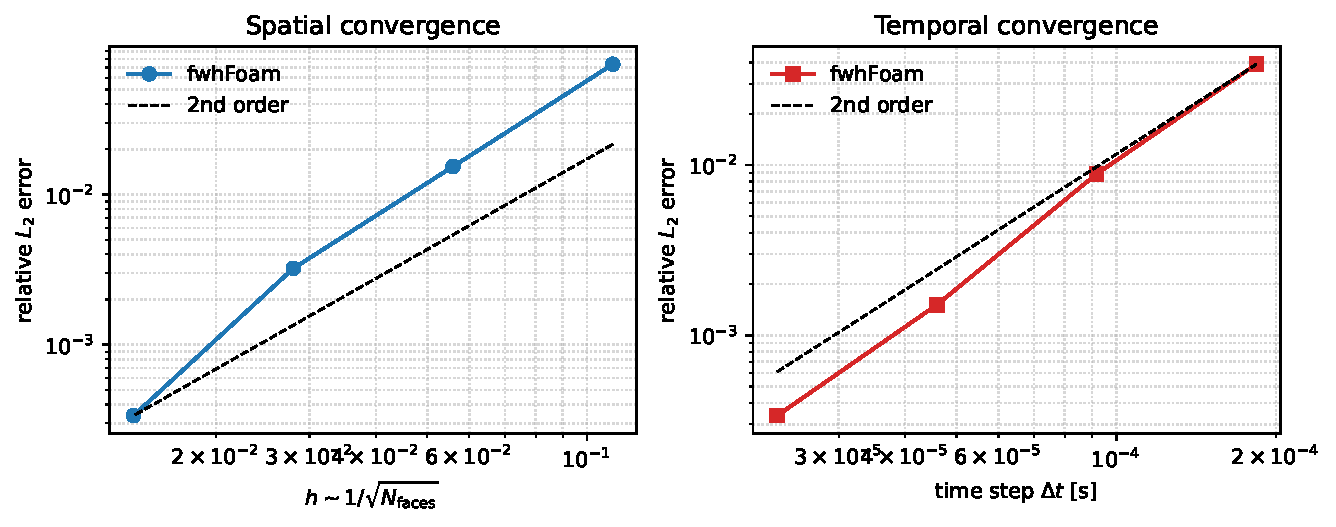
\includegraphics[width=0.85\linewidth]{figs/convergence.pdf}
\caption{Spatial (left) and temporal (right) convergence of the relative
$L_2$ error for the analytic monopole; dashed lines are second-order slopes.}
\label{fig:convergence}
\end{figure}

\subsection{Verification of the localization density}

The power identity underlying $\sigma$ is verified independently: for exact
monopole and dipole fields on a 1280-face icosphere, the analytic radiated
power, the far-field power and $\oint\sigma\,dS$ agree to $2.9\times10^{-3}$,
and $\sigma$ reproduces the correct spatial structure --- uniform for the
isotropic monopole, and vanishing at the poles while peaking at the equator
for the dipole ($\cos^2$ pattern).

\subsection{Aeolian tone and source map of a circular cylinder}

Laminar flow past a 2D cylinder at $Re=100$ (incompressible
\texttt{pimpleFoam}) sheds a von K\'arm\'an street, producing a lift-dipole
tone. The runtime \texttt{fwh} object on the cylinder wall recovers the tone
at the shedding Strouhal number $St=0.166$ (Fig.~\ref{fig:cylinder}), matched
against the lift-coefficient spectrum, with the expected dipole directivity.
Sampling instead on a permeable control surface of radius $8D$ and applying
\eqref{eq:sigma} at the tone yields the source map of Fig.~\ref{fig:sigma}:
the density concentrates on the downstream sector where the unsteady wake
crosses the surface, forms a signed lobe pair, and integrates to the
far-field power to machine precision --- the built-in identity holding on
genuine CFD data.

\begin{figure}[!h]
\centering
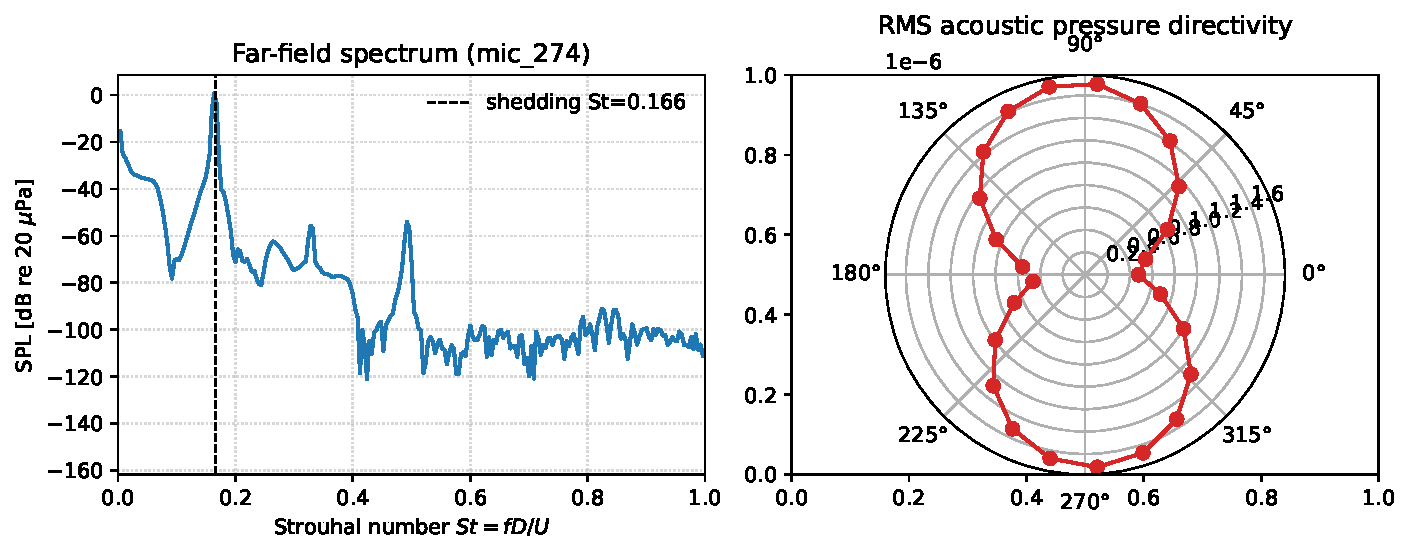
\includegraphics[width=0.85\linewidth]{figs/cylinder.pdf}
\caption{Cylinder Aeolian tone at $Re=100$: (left) far-field spectrum at the
cross-flow observer, peaking at the shedding Strouhal number; (right) RMS
acoustic-pressure directivity (lift-dipole lobes).}
\label{fig:cylinder}
\end{figure}

\begin{figure}[!h]
\centering
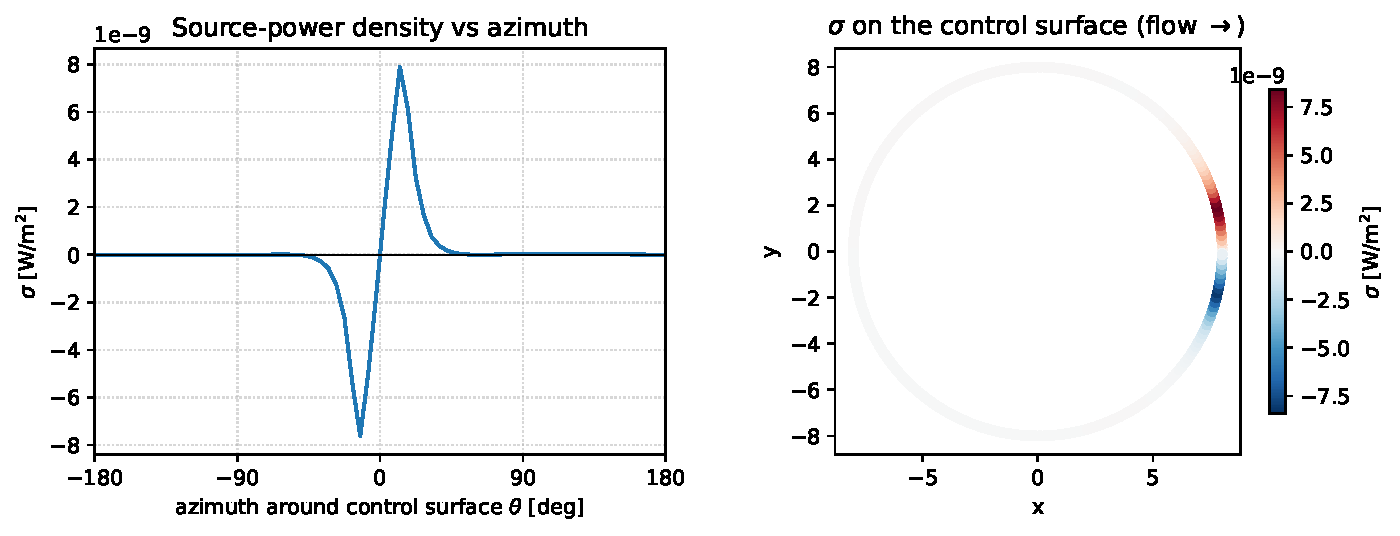
\includegraphics[width=0.85\linewidth]{figs/sigma_cylinder.pdf}
\caption{Source-power density $\sigma$ on the permeable control surface
($r=8D$) at the shedding tone: (left) azimuthal profile; (right) $\sigma$
over the surface (mean flow left to right). The signed density localizes the
radiating region; $\oint\sigma\,dS=P$ to machine precision.}
\label{fig:sigma}
\end{figure}

%% ------------------------------------------------------------------
\section{Impact}
\label{sec:impact}

As a far-field solver, \texttt{fwhFoam} provides a documented and verified
FW-H capability that complements existing libraries; the offline
\texttt{fwhSolve} utility separates the CFD from the acoustic
post-processing, so observer arrays, ambient conditions and mean-flow speeds
can be changed without re-running the flow solver. The surface sound-power
density $\sigma$ additionally turns an FW-H integration surface, normally
used only for a far-field signal, into a diagnostic of which surface regions
radiate. This is relevant to noise-reduction studies, where the location of
the sources on an airframe, edge or porous treatment matters and is not
available from a far-field spectrum alone~\cite{delfs2024}. Because $\sigma$
uses the same data as the FW-H integral and satisfies the power identity, it
adds this diagnostic without additional simulation and with an internal
check. The verification and convergence suites are reproducible, and the
mesh-independent engine is a basis for moving-surface and frequency-domain
extensions.

%% ------------------------------------------------------------------
\section{Conclusions}
\label{sec:conclusions}

\texttt{fwhFoam} is a Ffowcs Williams--Hawkings solver for OpenFOAM that
supports permeable and impermeable surfaces and a uniform mean flow, and that
computes the surface sound-power density $\sigma$ for on-surface source
localization from the same data as the far-field integral, subject to a power
identity used as an internal check. Far-field predictions are verified
against analytic solutions to about 0.1\,\% with second-order convergence,
and the localization density is verified through its power identity to a few
tenths of a percent. Planned extensions include moving and rotating
integration surfaces, the diffraction-filter projection for rigid-wall data,
and a frequency-domain formulation.

%% ------------------------------------------------------------------
\section*{Acknowledgements}

Computations were performed on the DLR CARA high-performance computing
cluster.

\begin{thebibliography}{00}

\bibitem{fwh1969} J.~E. Ffowcs Williams, D.~L. Hawkings, Sound generation by
turbulence and surfaces in arbitrary motion, Phil. Trans. R. Soc. A 264
(1151) (1969) 321--342.

\bibitem{difrancescantonio1997} A.~Di Francescantonio, A new boundary
integral formulation for the prediction of sound radiation, J. Sound Vib.
202 (4) (1997) 491--509.

\bibitem{brentner1998} K.~S. Brentner, F.~Farassat, Analytical comparison of
the acoustic analogy and Kirchhoff formulation for moving surfaces, AIAA J.
36 (8) (1998) 1379--1386.

\bibitem{farassat2007} F.~Farassat, Derivation of Formulations 1 and 1A of
Farassat, NASA TM-2007-214853, 2007.

\bibitem{casalino2003} D.~Casalino, An advanced time approach for acoustic
analogy predictions, J. Sound Vib. 261 (4) (2003) 583--612.

\bibitem{epikhin2015} A.~Epikhin, I.~Evdokimov, M.~Kraposhin, M.~Kalugin,
S.~Strijhak, Development of a dynamic library for computational aeroacoustics
applications using the OpenFOAM open source package, Procedia Computer
Science 66 (2015) 150--157.

\bibitem{delfs2024} J.~W. Delfs, B.~Ruck, A quantity to identify turbulence
related sound generation on surfaces, J. Sound Vib. 586 (2024) 118490.

\end{thebibliography}

\end{document}
